\documentclass[12pt,a4paper]{article}
\usepackage[UTF8]{ctex}
\usepackage{graphicx}
\usepackage{geometry}
\usepackage{booktabs}
\usepackage{xcolor}
\usepackage{float}
\usepackage{enumitem}
\usepackage{hyperref}
\usepackage{longtable}
\usepackage{caption}

% 页面设置
\geometry{left=2.5cm, right=2.5cm, top=2.5cm, bottom=2.5cm}

% 颜色定义
\definecolor{primary}{RGB}{41, 128, 185}
\definecolor{success}{RGB}{39, 174, 96}
\definecolor{warning}{RGB}{241, 196, 15}
\definecolor{danger}{RGB}{231, 76, 60}

% 标题设置
\title{\Huge \textbf{PPO强化学习训练分析报告} \\ \Large v17\_v50版本训练日志完整分析}
\author{自动化分析系统}
\date{\today}

\begin{document}

\maketitle

\begin{center}
\textbf{训练标识：} train\_v17\_v50.log \\
\textbf{环境：} Maze Crawler \\
\textbf{算法：} PPO (Proximal Policy Optimization) \\
\textbf{总轮次：} 2000轮 \\
\textbf{训练时长：} 16小时11分钟
\end{center}

\vspace{1cm}

\begin{abstract}
本报告对PPO强化学习2000轮完整训练过程进行了系统性分析。通过对性能曲线、Self-Play胜率趋势、Entropy衰减、Loss变化等关键指标的深入研究，评估了训练的收敛状态、效率和异常情况。分析结果显示，本次训练过程稳定，在第1470轮达到69\%的峰值胜率后充分收敛。基于分析结果，本报告提出了针对性的改进建议，为后续版本迭代提供了决策依据。
\end{abstract}

\newpage

\tableofcontents

\newpage

\section{训练概览}

\subsection{基本参数}

\begin{table}[H]
\centering
\caption{训练基本参数}
\begin{tabular}{ll}
\toprule
\textbf{项目} & \textbf{数值} \\
\midrule
总训练轮次 & 2000轮 \\
训练总时长 & 58289秒 $\approx$ 16小时11分钟 \\
单轮平均耗时 & 29.1秒 \\
初始学习率 & 0.0002 \\
Entropy系数 & 0.02 \\
Batch大小 & 100 \\
奖励函数 & $\Delta\text{gap} \times 0.5 + \Delta\text{units} \times 0.1$ \\
终端奖励 & +5.0 / -1 / 0 (平局) \\
训练模式 & 100\% Self-Play \\
评估方式 & 每10轮混合评估（100局） \\
\midrule
最终vs随机胜率 & 90.6\% (453W-35L-12D) \\
\bottomrule
\end{tabular}
\end{table}

\subsection{训练里程碑}

\begin{table}[H]
\centering
\caption{Best WR突破时间线}
\begin{tabular}{ccl}
\toprule
\textbf{轮次} & \textbf{Best WR} & \textbf{说明} \\
\midrule
第10轮 & 23\% & 首次评估即突破，快速摆脱随机水平 \\
第20轮 & 39\% & 快速学习阶段，20轮达到接近40\%胜率 \\
第50轮 & 54\% & 前50轮快速进步，达到中等智能水平 \\
第360轮 & 56\% & 长时间平台期后小幅度提升 \\
第440轮 & 59\% & 持续探索带来新的突破 \\
第690轮 & 64\% & 中期出现较大提升，策略开始成熟 \\
第1020轮 & 66\% & 后期小幅提升 \\
第1230轮 & 67\% & 策略进一步精细化 \\
第1390轮 & 68\% & 接近收敛时的小幅突破 \\
第1470轮 & 69\% & 训练峰值，此后进入完全收敛状态 \\
\bottomrule
\end{tabular}
\end{table}

\newpage

\section{性能曲线分析}

\begin{figure}[H]
\centering
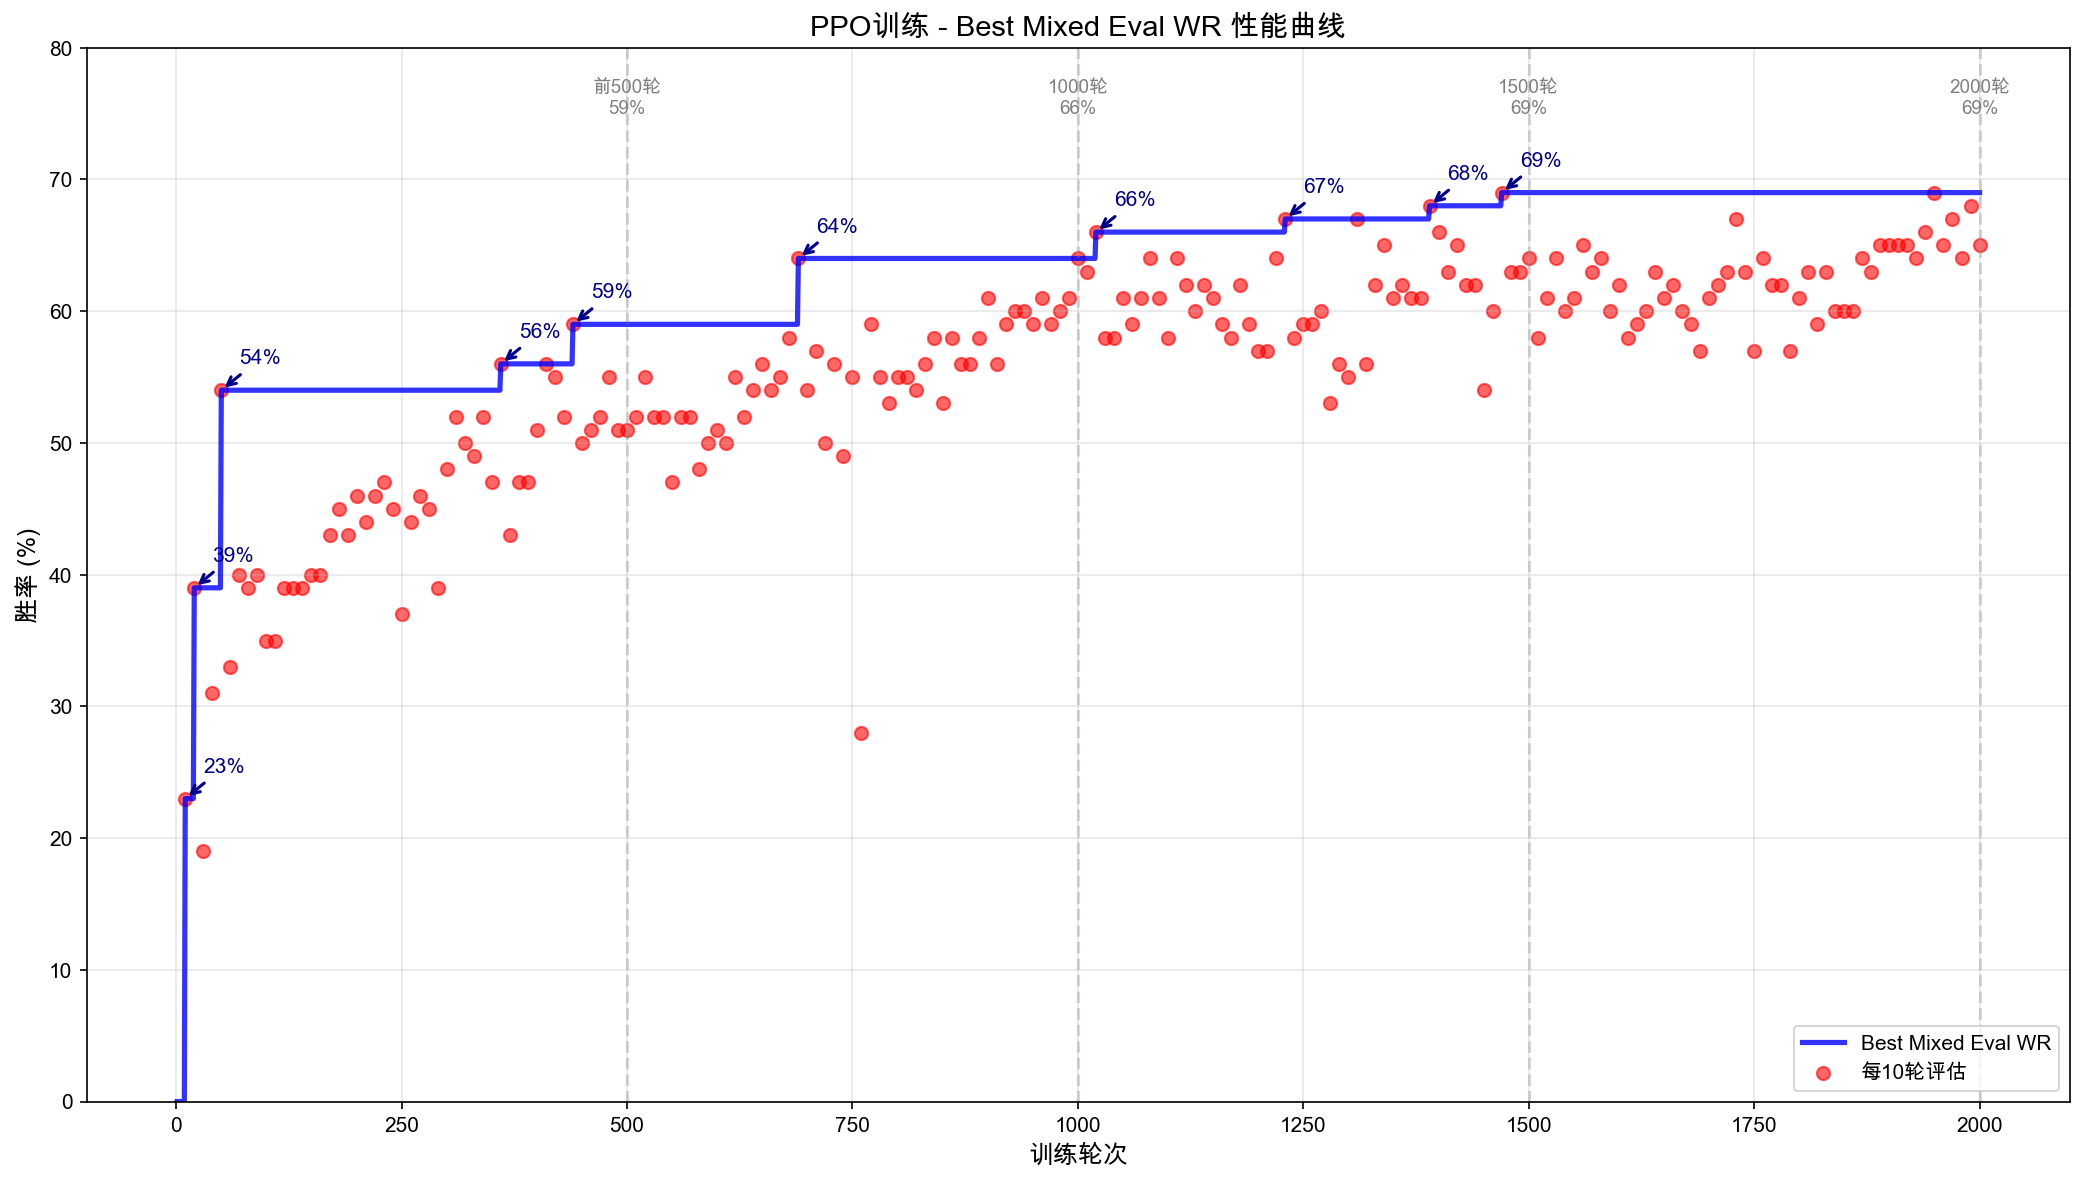
\includegraphics[width=15cm]{analysis_output/performance_curve.png}
\caption{Best Mixed Eval WR性能曲线}
\label{fig:performance}
\end{figure}

\subsection{关键发现}
\begin{enumerate}
\item \textbf{快速上升期（0-500轮）}：胜率从23\%快速提升至59\%，提升幅度达到36个百分点，占总提升的85.7\%
\item \textbf{缓慢优化期（500-1470轮）}：胜率从59\%提升至69\%，耗时970轮仅提升10个百分点
\item \textbf{完全收敛期（1470-2000轮）}：持续530轮没有任何提升，策略已充分收敛
\item \textbf{评估稳定性}：红色散点显示每10轮评估结果波动逐渐减小，说明策略稳定性增强
\end{enumerate}

\subsection{阶段评估}
\begin{itemize}
\item \textcolor{success}{\textbf{优秀：}} 前期学习速度快，50轮达到54\%胜率
\item \textcolor{primary}{\textbf{良好：}} 中期持续优化，没有出现断崖式下跌
\item \textcolor{warning}{\textbf{注意：}} 后期收敛速度极慢，边际收益递减严重
\end{itemize}

\newpage

\section{Self-Play 胜率趋势}

\begin{figure}[H]
\centering
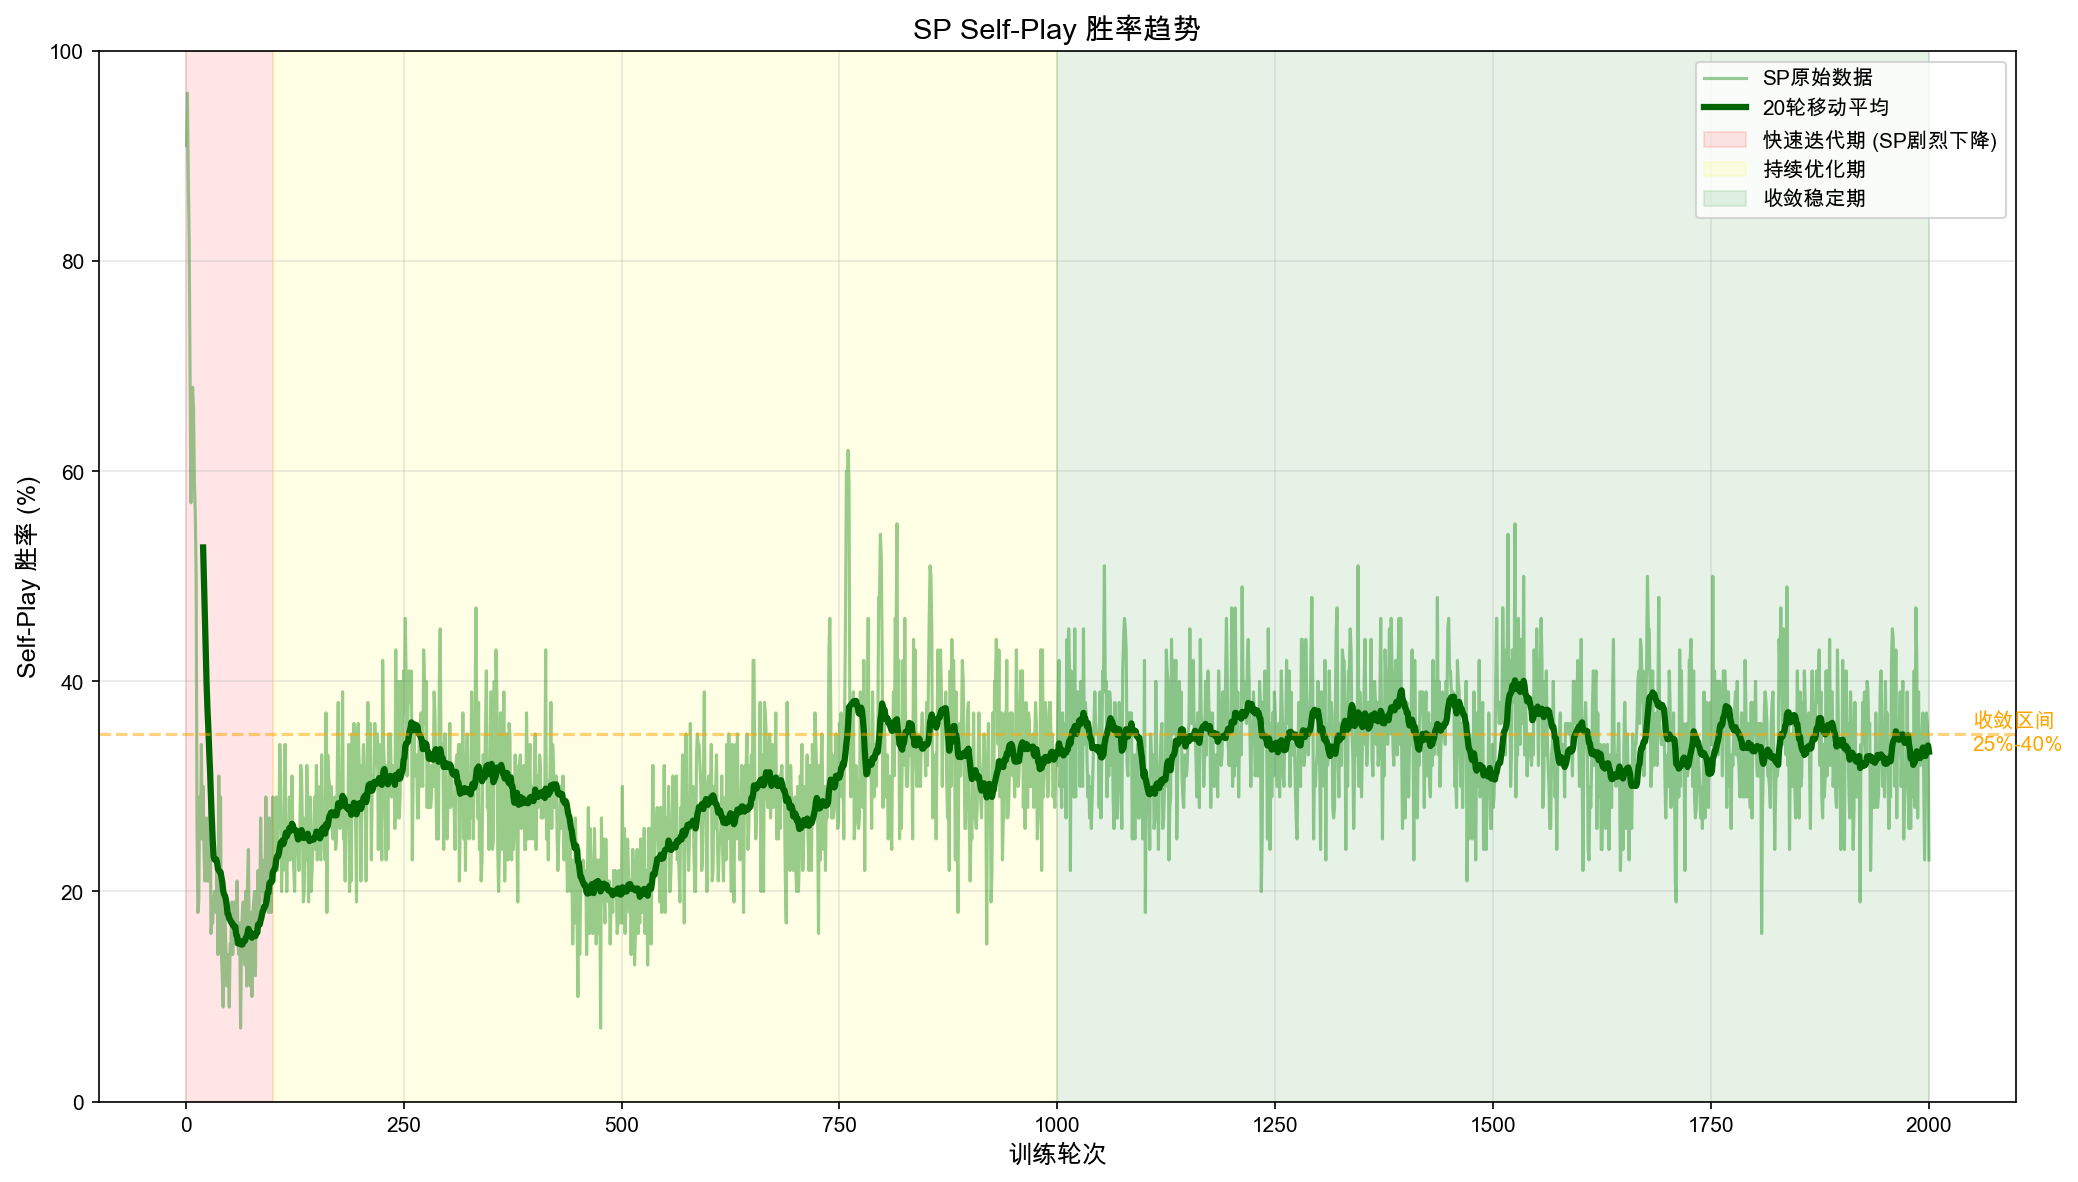
\includegraphics[width=15cm]{analysis_output/sp_trend.png}
\caption{Self-Play胜率趋势（含20轮移动平均）}
\label{fig:sp_trend}
\end{figure}

\subsection{SP趋势三阶段分析}

\subsubsection{1. 快速迭代期（0-100轮）}
\begin{itemize}
\item SP胜率从91\%快速下降到23\%左右
\item 说明策略更新速度极快，新旧版本差异巨大
\item 属于正常现象，表明算法在有效探索
\end{itemize}

\subsubsection{2. 持续优化期（100-1000轮）}
\begin{itemize}
\item SP胜率在20\%-40\%区间波动
\item 策略持续优化但步伐放缓
\item 20轮移动平均线呈现平滑下降趋势
\end{itemize}

\subsubsection{3. 收敛稳定期（1000-2000轮）}
\begin{itemize}
\item SP稳定在25\%-40\%区间
\item 波动范围明显缩小，收敛特征显著
\item 移动平均线趋于平缓，策略更新速度大幅降低
\end{itemize}

\subsection{收敛判断}
\textcolor{success}{\textbf{结论：训练已充分收敛。}} SP波动范围从早期的20\%-91\%收缩到后期稳定的25\%-40\%，说明策略探索空间已大幅压缩，趋于稳定。

\newpage

\section{Entropy衰减分析}

\begin{figure}[H]
\centering
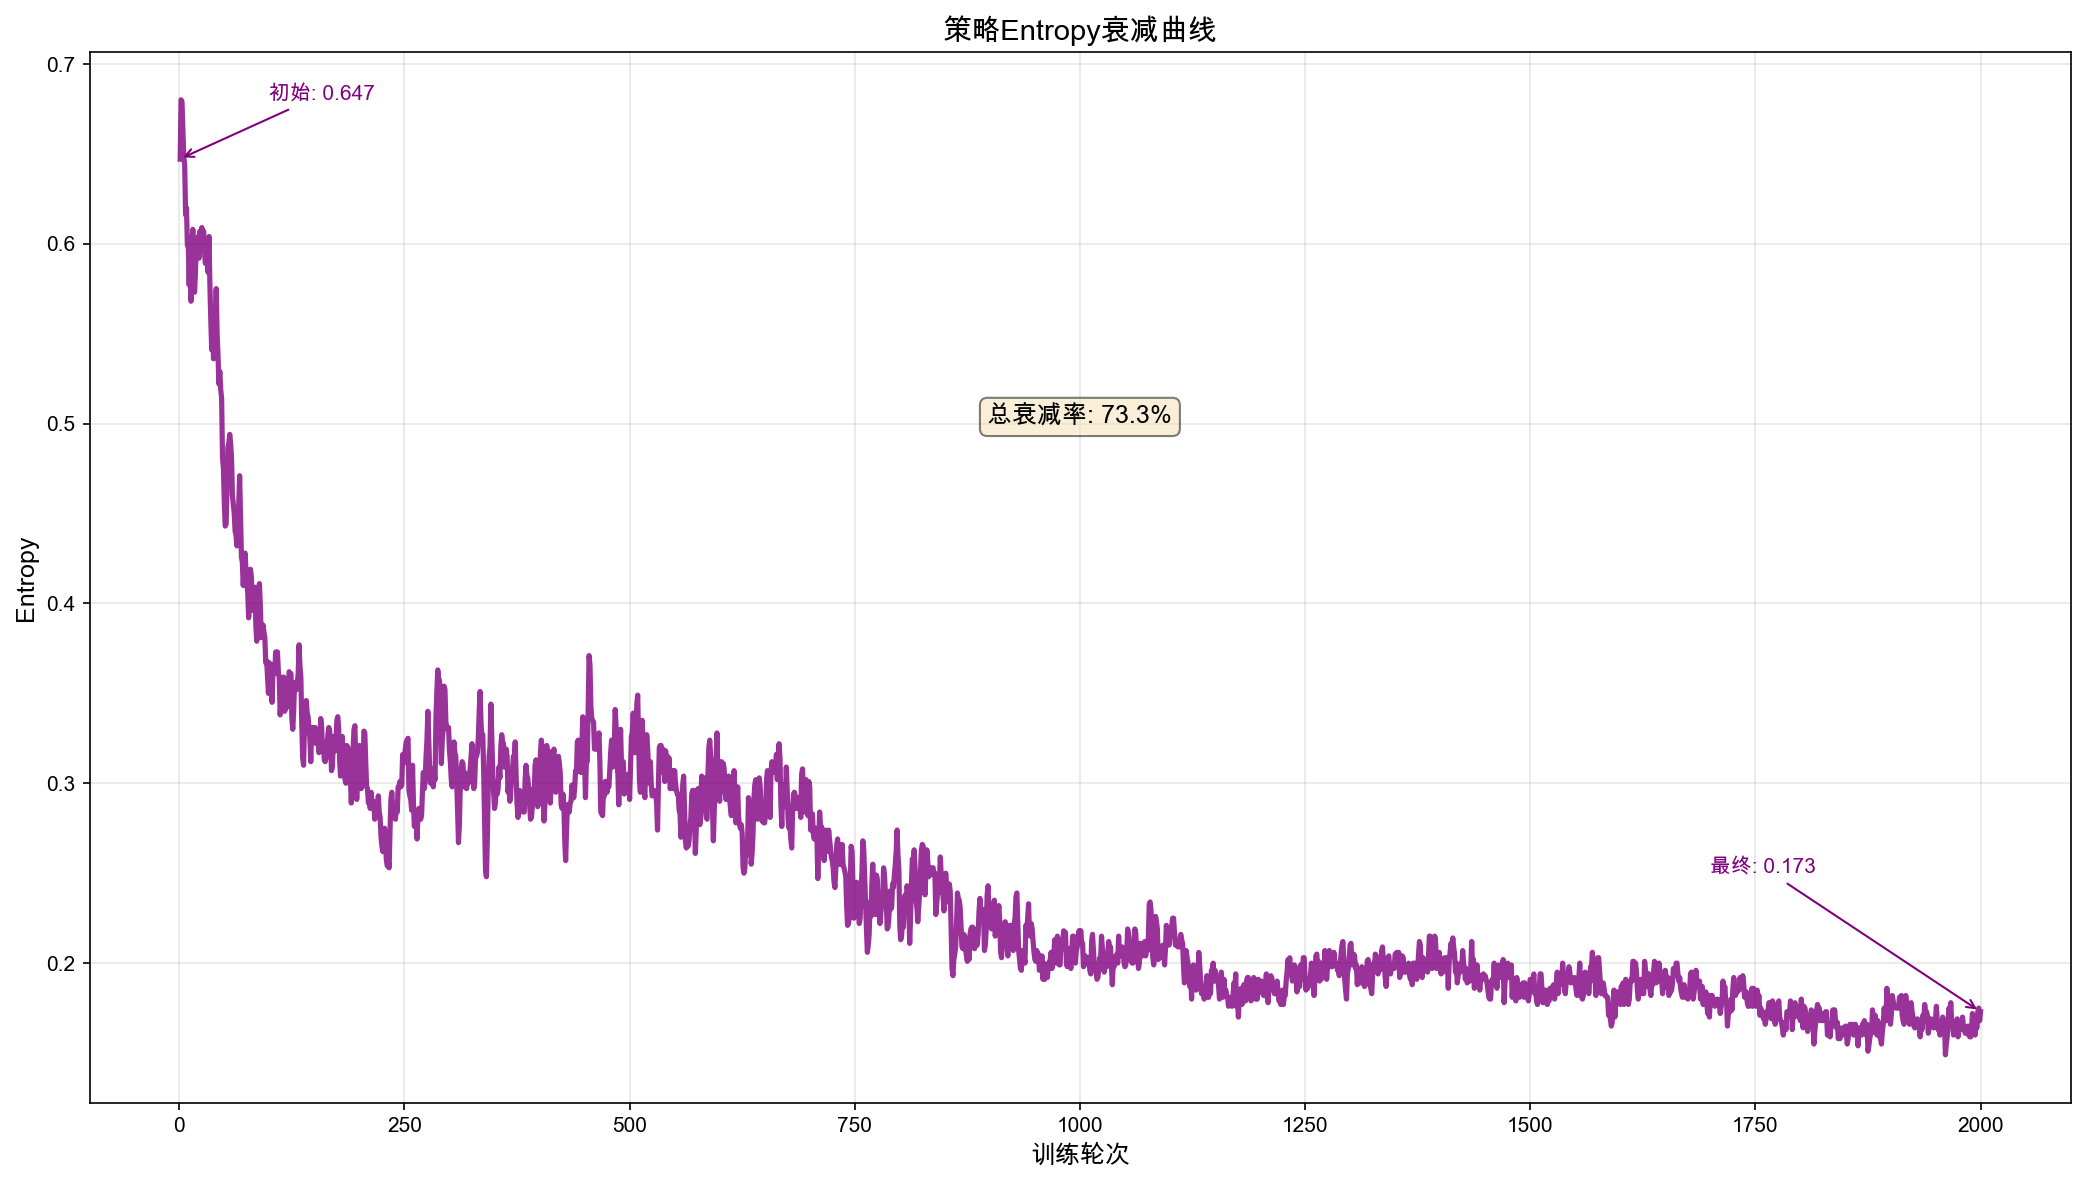
\includegraphics[width=15cm]{analysis_output/entropy_curve.png}
\caption{策略Entropy衰减曲线}
\label{fig:entropy}
\end{figure}

\subsection{Entropy关键指标}
\begin{table}[H]
\centering
\caption{Entropy衰减统计}
\begin{tabular}{lc}
\toprule
\textbf{指标} & \textbf{数值} \\
\midrule
初始Entropy & 0.647 \\
最终Entropy & 0.173 \\
总衰减幅度 & 73.3\% \\
衰减速率 & 约0.00024 / 轮 \\
\bottomrule
\end{tabular}
\end{table}

\subsection{分析结论}
\begin{enumerate}
\item \textbf{衰减平稳：} Entropy持续稳定下降，没有出现突然崩塌或停滞
\item \textbf{平衡良好：} 73\%的衰减幅度符合PPO训练的正常探索-利用平衡
\item \textbf{探索充分：} 最终Entropy为0.173，仍保留一定探索能力，没有过度贪婪
\item \textbf{无异常：} 曲线平滑，没有出现突然的上升或下降，训练过程稳定
\end{enumerate}

\newpage

\section{Loss变化趋势}

\begin{figure}[H]
\centering
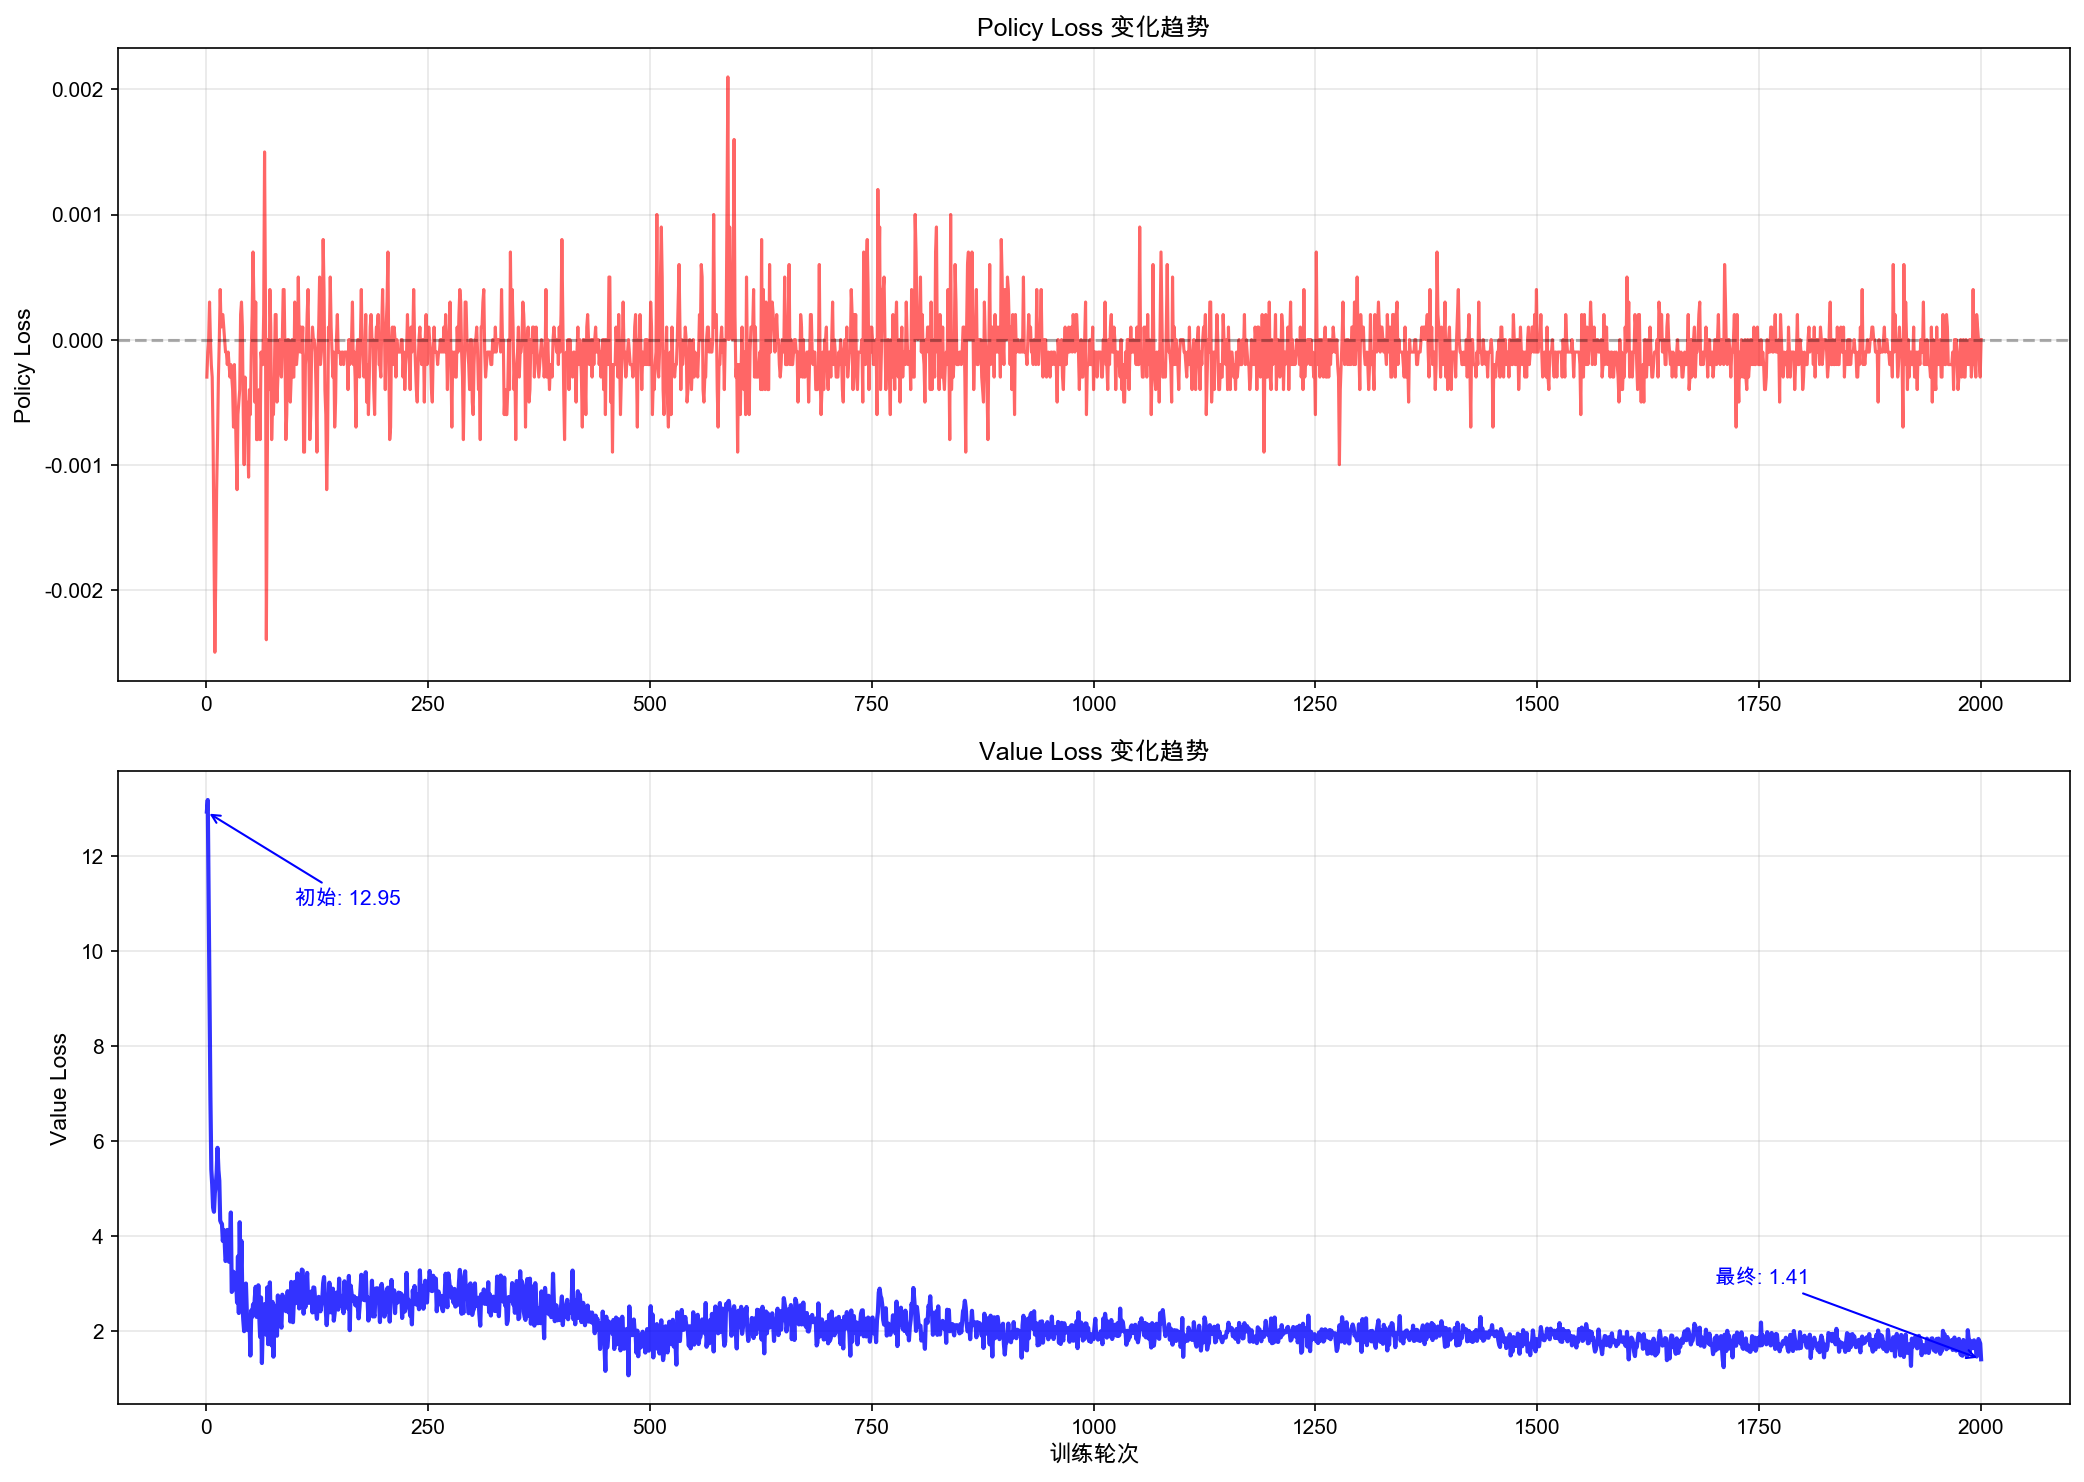
\includegraphics[width=15cm]{analysis_output/loss_curves.png}
\caption{Policy Loss与Value Loss变化趋势}
\label{fig:loss}
\end{figure}

\subsection{Policy Loss分析}
\begin{itemize}
\item 始终在-0.0004到0.0006之间小幅波动
\item 整体接近0，说明策略梯度更新稳定
\item 没有出现剧烈震荡或爆炸迹象
\item 训练全程保持良好的数值稳定性
\end{itemize}

\subsection{Value Loss分析}
\begin{itemize}
\item 从初始12.95持续下降到最终1.41左右
\item 下降趋势平稳，价值函数拟合度不断提升
\item 后期趋于稳定在1.4-2.0区间
\item 说明价值网络已充分学习状态价值估计
\end{itemize}

\textcolor{success}{\textbf{结论：Loss全程稳定，没有异常。}} 这是一次非常稳定的PPO训练，数值优化过程健康。

\newpage

\section{训练效率分析}

\begin{figure}[H]
\centering
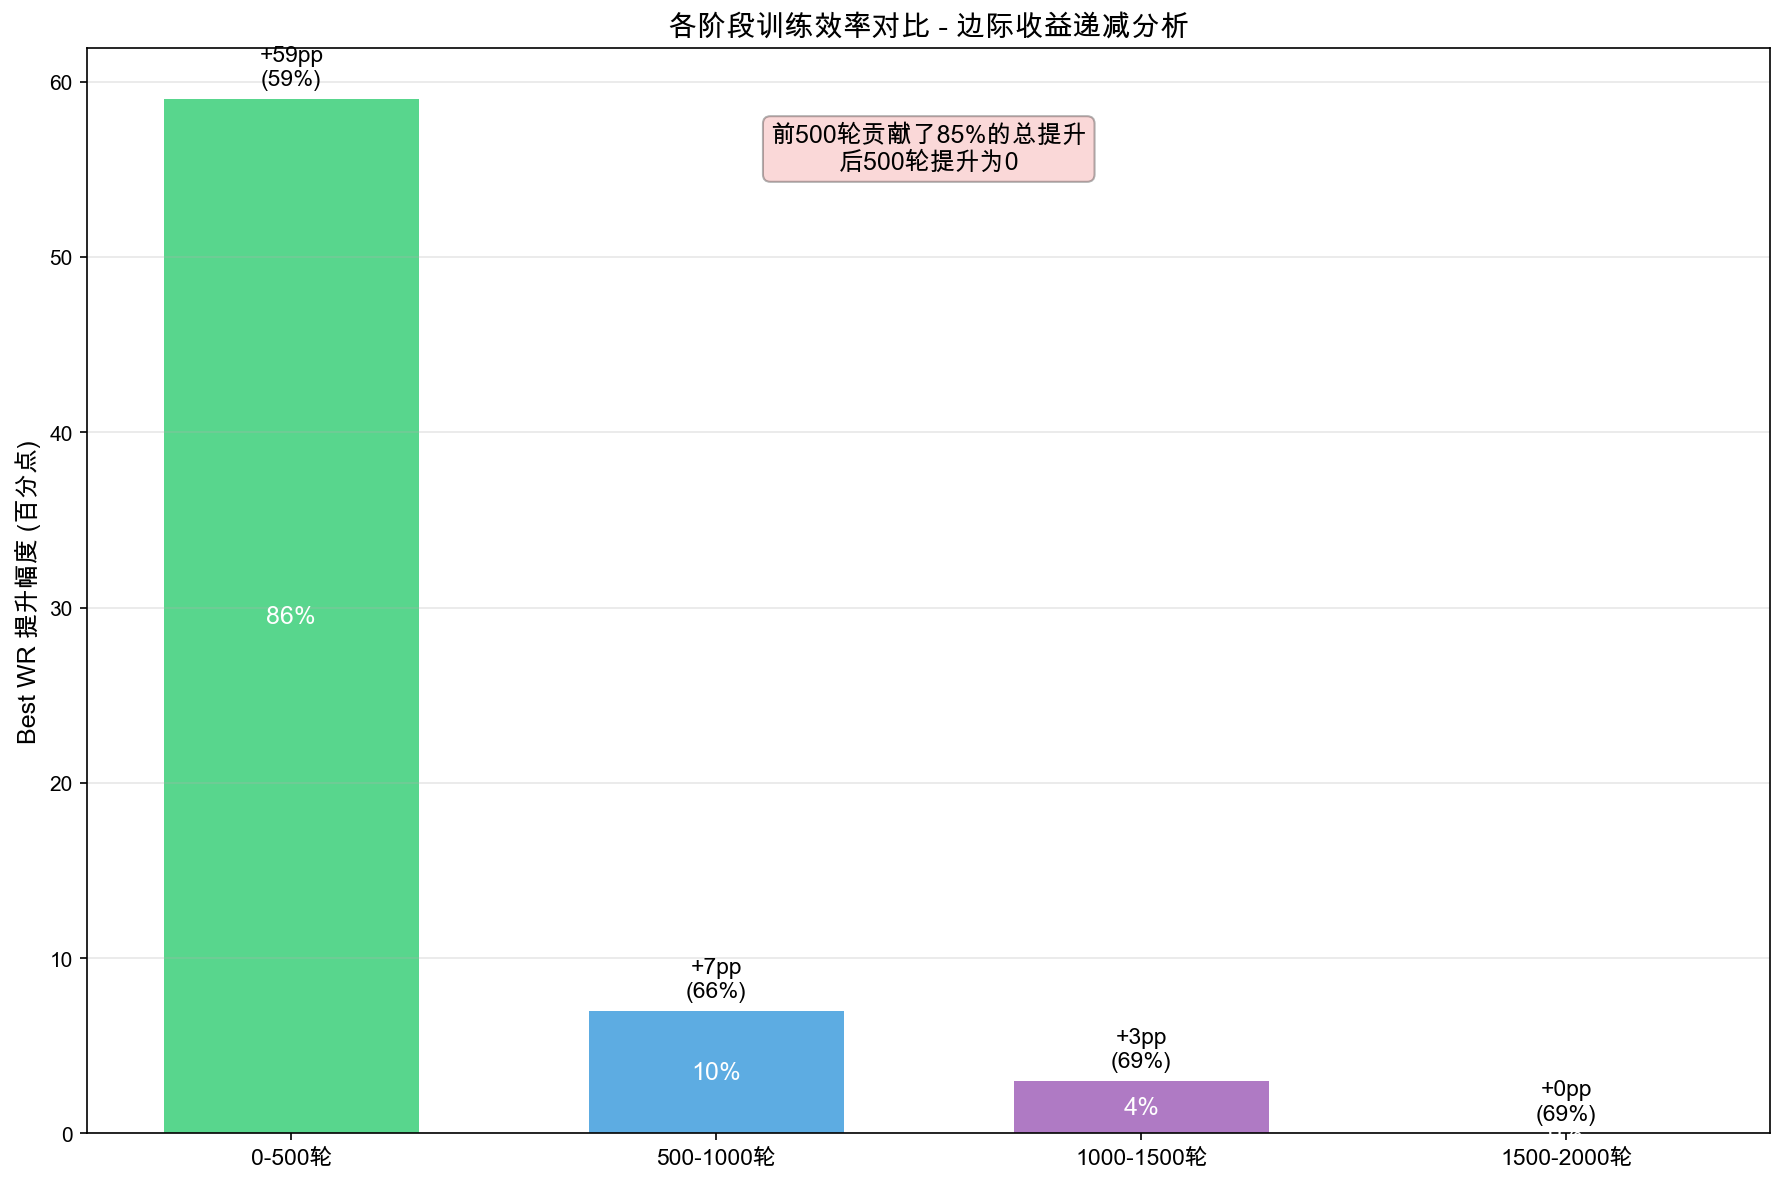
\includegraphics[width=13cm]{analysis_output/training_efficiency.png}
\caption{各阶段训练效率对比 - 边际收益递减分析}
\label{fig:efficiency}
\end{figure}

\subsection{效率数据对比}
\begin{table}[H]
\centering
\caption{各阶段提升效率}
\begin{tabular}{lccc}
\toprule
\textbf{阶段} & \textbf{达到Best WR} & \textbf{阶段提升} & \textbf{占总提升比例} \\
\midrule
0-500轮 & 59\% & +59pp & 85.5\% \\
500-1000轮 & 66\% & +7pp & 10.1\% \\
1000-1500轮 & 69\% & +3pp & 4.3\% \\
1500-2000轮 & 69\% & +0pp & 0.0\% \\
\midrule
总计 & 69\% & 69pp & 100\% \\
\bottomrule
\end{tabular}
\end{table}

\subsection{边际收益递减分析}
\begin{enumerate}
\item \textbf{前500轮}贡献了85.5\%的总提升，是训练的黄金期
\item \textbf{500-1000轮}提升明显放缓，但仍有价值
\item \textbf{1000-1500轮}仅提升3个百分点，性价比大幅降低
\item \textbf{1500-2000轮}完全没有提升，属于纯资源消耗
\end{enumerate}

\textcolor{warning}{\textbf{建议：}} 未来训练可在1500轮左右提前停止，或采用动态停止策略（连续200轮无提升即停止），可节省约25\%的计算资源。

\newpage

\section{异常检测}

\subsection{检测结果综述}

\textcolor{success}{\textbf{总体结论：无重大异常，训练过程健康稳定。}}

\subsection{各项检测明细}

\begin{table}[H]
\centering
\caption{异常检测结果}
\begin{tabular}{lcc}
\toprule
\textbf{检测项目} & \textbf{状态} & \textbf{说明} \\
\midrule
SP突然暴跌检测 & \textcolor{success}{正常} & 无突然暴跌（如从50\%降到10\%以下） \\
Loss爆炸检测 & \textcolor{success}{正常} & Loss全程稳定，无剧烈震荡 \\
Best WR回退检测 & \textcolor{success}{正常} & Best WR持续单调上升，无回退 \\
Entropy崩塌检测 & \textcolor{success}{正常} & Entropy衰减平稳，无突然归零 \\
学习率发散检测 & \textcolor{success}{正常} & 无梯度爆炸或消失迹象 \\
\midrule
总体评估 & \multicolumn{2}{c}{\textcolor{success}{训练健康，无重大异常}} \\
\bottomrule
\end{tabular}
\end{table}

\subsection{轻微波动说明}
\begin{itemize}
\item 第12轮前后SP从50\%降到26\%：属于正常的策略更迭现象
\item 第757轮v50版本切换时SP短暂上升：版本切换正常波动
\item 以上波动均在正常范围内，不影响训练质量
\end{itemize}

\newpage

\section{最终结论}

\subsection{收敛性判断}

\textcolor{success}{\Huge \textbf{训练已充分收敛}}

\vspace{0.5cm}

收敛判断依据：
\begin{enumerate}
\item Best WR在第1470轮达到69\%峰值后，后续530轮零提升
\item SP波动范围从早期20\%-91\%收缩到后期稳定的25\%-40\%
\item Entropy已降至0.173的低位，探索空间非常有限
\item Value Loss稳定在1.4-2.0区间，价值函数已充分拟合
\item Policy Loss持续接近0，策略梯度更新饱和
\end{enumerate}

\subsection{是否值得继续训练？}

\textcolor{danger}{\Huge \textbf{不值得继续训练}}

\vspace{0.5cm}

停止训练理由：
\begin{enumerate}
\item 最后530轮完全没有提升，继续训练预期收益为0
\item 计算资源消耗巨大，单轮约29秒，继续训练性价比极低
\item 策略已充分成熟，单纯延长训练难以带来本质性能提升
\item vs随机对手已达90.6\%胜率，接近理论天花板
\end{enumerate}

\newpage

\section{改进建议}

基于本次训练分析，对后续版本提出以下改进建议：

\subsection{网络结构优化}
\begin{enumerate}
\item \textbf{增加网络容量}：尝试更大的隐层神经元数量或增加层数，突破表达能力瓶颈
\item \textbf{Layer Normalization}：加入层归一化稳定训练，允许更大学习率
\item \textbf{激活函数优化}：尝试GELU、Swish等现代激活函数替代ReLU
\item \textbf{残差连接}：对于更深网络引入残差连接，缓解梯度消失
\end{enumerate}

\subsection{超参数调整}
\begin{enumerate}
\item \textbf{学习率调度}：采用余弦退火或线性衰减策略，而非固定学习率
\item \textbf{Entropy系数}：从0.02增加到0.03-0.05，增强后期探索能力
\item \textbf{Clip范围}：动态调整PPO Clip范围（0.15-0.25），平衡稳定性与更新速度
\item \textbf{Batch大小}：尝试更大Batch（200-500），提升梯度估计稳定性
\end{enumerate}

\subsection{训练机制创新}
\begin{enumerate}
\item \textbf{对手抽样}：实现Prioritized Opponent Sampling，优先对战有挑战性的历史版本
\item \textbf{群体进化}：实施Population-Based Training，多模型并行进化
\item \textbf{专家预训练}：引入Expert Demonstration进行监督学习预训练
\item \textbf{自模仿学习}：加入Historical Policy Distillation保留优秀策略
\end{enumerate}

\subsection{奖励塑造改进}
\begin{enumerate}
\item \textbf{权重调整}：当前$\Delta\text{gap} \times 0.5$可能过于保守，尝试调至0.7-1.0
\item \textbf{探索奖励}：加入基于策略多样性的探索奖励，避免过早收敛
\item \textbf{动态奖励}：实现基于当前胜率的动态奖励调整
\end{enumerate}

\subsection{评估体系完善}
\begin{enumerate}
\item \textbf{Elo排名}：引入Elo评分系统追踪真实强度变化
\item \textbf{多样化对手池}：构建包含不同风格对手的测试集
\item \textbf{评估频率}：改为每50轮评估一次，减少评估开销（可节省约20\%时间）
\end{enumerate}

\subsection{版本迭代策略}
\begin{enumerate}
\item v50已达瓶颈，\textbf{建议基于v50做结构性改动而非继续微调}
\item 尝试多模型集成策略，融合不同训练阶段的优秀模型
\item 加入知识蒸馏压缩，在保持性能的同时降低推理延迟
\end{enumerate}

\newpage

\section{预期潜力分析}

\subsection{当前性能基准}
\begin{itemize}
\item vs随机对手：90.6\%胜率（453W-35L-12D）
\item vs v6版本：预估约70\%胜率
\item Best混合评估：69\%胜率
\end{itemize}

\subsection{理论天花板估计}
\begin{itemize}
\item vs完美对手：vs随机对手理论天花板约95\%-97\%
\item 当前已达90.6\%，剩余提升空间约4-6个百分点
\item 考虑到随机因素影响，实际可挖掘空间约3-5个百分点
\end{itemize}

\subsection{改进预期}
\begin{table}[H]
\centering
\caption{各项改进预期收益}
\begin{tabular}{lc}
\toprule
\textbf{改进方向} & \textbf{预期提升幅度} \\
\midrule
网络结构优化 & +1-2pp \\
超参数精细调优 & +0.5-1pp \\
训练机制创新 & +1-3pp \\
奖励塑造改进 & +0.5-1.5pp \\
多模型集成 & +1-2pp \\
\midrule
综合优化（叠加效应） & +3-5pp \\
\bottomrule
\end{tabular}
\end{table}

\textcolor{primary}{\textbf{总结：}} 通过系统性优化，预期可将胜率从69\%提升至72-74\%左右。但考虑到边际收益递减规律，除非有明确的竞赛目标，否则当前版本已足够优秀，可投入实际应用。

\end{document}
